% !TEX root = ../thesis.tex

\chapter{Concepts}
\label{sec:concepts}

% \cleanchapterquote{Users do not care about what is inside the box, as long as the box does what they need done.}{Jef Raskin}{about Human Computer Interfaces}

Here I give non-exhaustive explanations for general concepts that I find useful to understand related work.

\begin{description}

  \item[Perceptual quality]
  A user-oriented metric used for evaluating picture quality.
  It is usually evaluated by subjective tests with standard procedures run on several viewers. \cite{Lin2011}

  \item[Overfitting]
  TODO
  \todo[inline]{}

  \item[Perceptron]
  A binary classifier regardless of how it is implemented. It may very well be just a function or a whole deep neural network.

  \item[Pooling layer]
  A method for reducing spatial size of the representation of the input.

  \item[Weight layer]
  TODO
  \todo[inline]{}

  \item[Ground Truth]
  TODO
  \todo[inline]{}

  \item[Back-propagation]
  TODO
  \todo[inline]{}

  \item[Convolution]
  \todo{More info}In image processing, convolution is a process that transforms an image.

  \item[Feature learning]
  Finding kernel that produce the desired feature maps is very difficult since it greatly varies depending on the task.
  In CNN, feature learning is the step in which the kernel gets increasingly better at the task of filtering an image or a feature map coming from a previous layer.

  \item[ImageNet]
  A large-scale, comprehensive and diverse database of accurately human-annotated images organized in a semantic hierarchy \cite{Deng2009} and it has become one of the main datasets in the field of object recognition.
  It it, each noun in English, coming from the lexical database WordNet \cite{Wilkniss1998}, is associated with hundreds of clean high-resolution images.
  These images depict different representations of the concepts or different perspectives and lighting conditions of the objects.
  The hierarchical structure of the database makes it possible to interlink concepts, allowing algorithms to recognizing several concepts at the same time (dog/mammal/animal).
  Its creation was motivated by the need to organize the huge amount of image data available on the Internet and make it available and useful to researchers of computer vision.

  \item[ImageNet Large-Scale Visual Recognition Challenge]
  The de-facto benchmark for large-scale object recognition algorithms \cite{Russakovsky2015}.
  It is run as a yearly competition since 2010 and has been one of the accelerators of the improvement of object recognition algorithms.
  The competition provides a publicly available dataset all algorithms have to classify to facilitate a standard evaluation between contending algorithms.
  A workshop is also organized to share results and discuss the strategies of the most accurate and innovative algorithms each year.

  \item[Deep learning framework]
  A deep learning framework is a piece of software that aims to provide a set of tools to design deep neural networks.
  They effectively separate the implementation of the network from its model.
  This has proved crucial for sharing trained models among researchers, helping the enthusiasm for deep neural networks.
  Some of the most popular ones currently are: TensorFlow, developed by Google \cite{Abadi2015}; Theano, developed by l’Université de Montréal \cite{Bergstra2010}; Caffe, developed by the Berkeley Vision and Learning Center \cite{Jia2014}; or Torch, supported by Facebook and Nvidia \cite{Collobert2002}.
\end{description}


% ------------------------------------------------------------------------------

\section{Types of Neural Networks}
\label{sec:Types of Neural Networks}

\begin{description}
  \item[Feed-forward Neural Networks]
  The simplest type of artificial neural network, characterized by its connections not forming cycles and thus the data always flowing in one direction: from input to hidden layers to output.

  \item[Multi-layer perceptron]
  It's a type of feed-forward neural network composed of several layers where neurons of one layer are fully connected with the next one.
  These neural networks are normally used to classify different inputs.
\end{description}


% ------------------------------------------------------------------------------

\section{Convolutional Neural Networks}
\label{sec:concepts:convolutional-neural-networks}
Convolutional Neural Networks, also known as CNNs or ConvNets, are feed-forward multi-layer neural networks inspired by the cat's visual ventral stream \cite{Hubel1968,Lawrence1997} and are responsible for a major breakthroughs in image recognition \cite{LeCun1995}.
They are able to learn patterns in images from a training set through back-propagation and present built-in resilience towards translation and distortion variances.
Such resilience minimizes pre-processing tasks both for training and classification and greatly reduces human supervision, making CNNs the currently preferred system for image recognition.

Although multi-layer perceptron are able to perform image recognition, they can only handle images of very small resolution due to the architectural limitations of fully connected layers \cite{ZHANG1999}.
Fully connected layers scale poorly, since neurons of the first hidden layer will process the whole image and will need to store weights for every color channel of every pixel.
Just to give a sense of the scale we are talking, for an RGB image of ${N}\times{M}$ pixels every neuron in a multi-layer perceptron will require storing ${N}\times{M}\times{3}$ weights, which for a ${32}\times{32}$ image it is $3072$ weights, but for a ${1024}\times{1024}$ one is more than $3$ millions.
In the shallower networks, with a single hidden layer, this already implies an exponential memory growth $O(N^2)$ with respect to image resolution.
Not only this is a performance issue in terms of hardware resources, the huge amount of parameters that need to be set also causes the system to quickly overfit.
Worse than that, treating pixels individually as described, regardless of their proximity, does not take into account the spatial information of an image.
That means that to handle variations in the images the network will end up with the same weights being stored in different neurons, proving multi-layer perceptron clearly inefficient for image recognition.
These problems are addressed by CNN architectural features \cite{LeCun1998}: 1) local receptive fields, 2) shared weights, and 3) subsampling.

\textbf{Local receptive fields} means taking into account spatial correlation, each neuron processing a small region of the image, the perceptive field, and it allows them to extract the most basic visual features such as edges, end-points or corners.
This architecture allows neurons in subsequent layers to, from those elementary visual features, extract progressively higher-order features like shapes, textures, faces or objects.
Within a layer several neurons performing different feature detections can can be stacked to receive the input from the perceptive field as depicted in Figure~\ref{fig:sec:concepts:conv-layer-1}.

\begin{figure}[htb]
  \begin{center}
    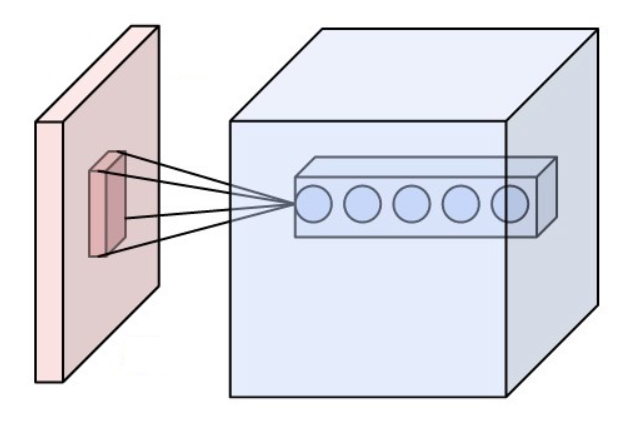
\includegraphics[width=0.5\textwidth]{gfx/conv-layer-1}
  \end{center}
  \caption{Stack of neurons applying different feature detections within a convolutional layer on the same perceptual region \cite{Aphex342015}.}
  \label{fig:sec:concepts:conv-layer-1}
\end{figure}

Layers in CNNs are organized in several slices, each of them containing neurons that detect the same feature but in different regions of the image and each slice detecting different features.
This operation is equivalent to a convolution in image processing, a sliding window that applies a transformation the original image, and that is where CNNs receive their name.
In this analogy, the kernel of the convolution is the filter applied by the slice over the input, represented by \textbf{weights shared} by all its neurons, being this what makes feature recognition robust against translations or distortions in the image.
The output of the convolution is referred to as \emph{feature map}, and all \emph{feature maps} produced by a convolutional layer together become the input for the next layer.
This is depicted in Figure~\ref{fig:sec:concepts:conv-layer-2}.

\begin{figure}[htb]
  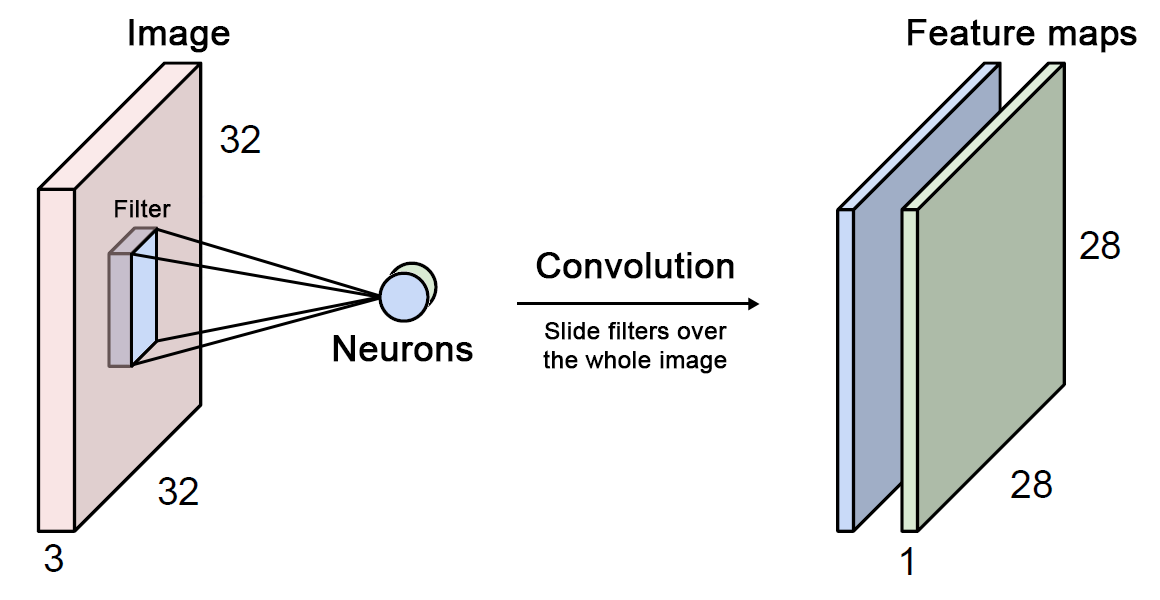
\includegraphics[width=\textwidth]{gfx/conv-layer-2}
  \caption{Anatomy of a convolutional layer and its output \cite{Guerzhoy2016}. On the left there is the representation of an image of ${32}\times{32}$ pixels with $3$ channels (\emph{RGB}). Neurons apply a filter of size ${5}\times{5}\times{3}$ in particular region of the image. Neurons of the same color belong to the same slice apply the same filter in different regions of the image and produce a \emph{feature map}. All \emph{feature maps} combined become the \"new image\" of size ${28}\times{28}\times{N}$, being $N$ the number of slices in the layer, that gets fed to the next layer.}
  \label{fig:sec:concepts:conv-layer-2}
\end{figure}

In the process of detecting higher-order features throughout subsequent layers of the network the exact absolute position of detected features in \emph{feature maps} is pretty much irrelevant compared to the relative position between them.
For instance, the pattern that describes the number $7$ is an endpoint in upper left area of a horizontal segment, a corner in the upper right area and an endpoint at the bottom of a vertical segment.
Still, small variations in the input may cause the pattern not to be detected because the features will not completely match the filter.
To make the network more robust against variations the sensitivity of the convolutional layers has to be reduced.
This is effectively accomplished by reducing the resolution of the feature maps through \textbf{subsampling} with pooling layers.
Pooling layers


% It's important to note that all the weights in the network are learnt through back-propagation.


\begin{figure}[htb]
  \begin{center}
    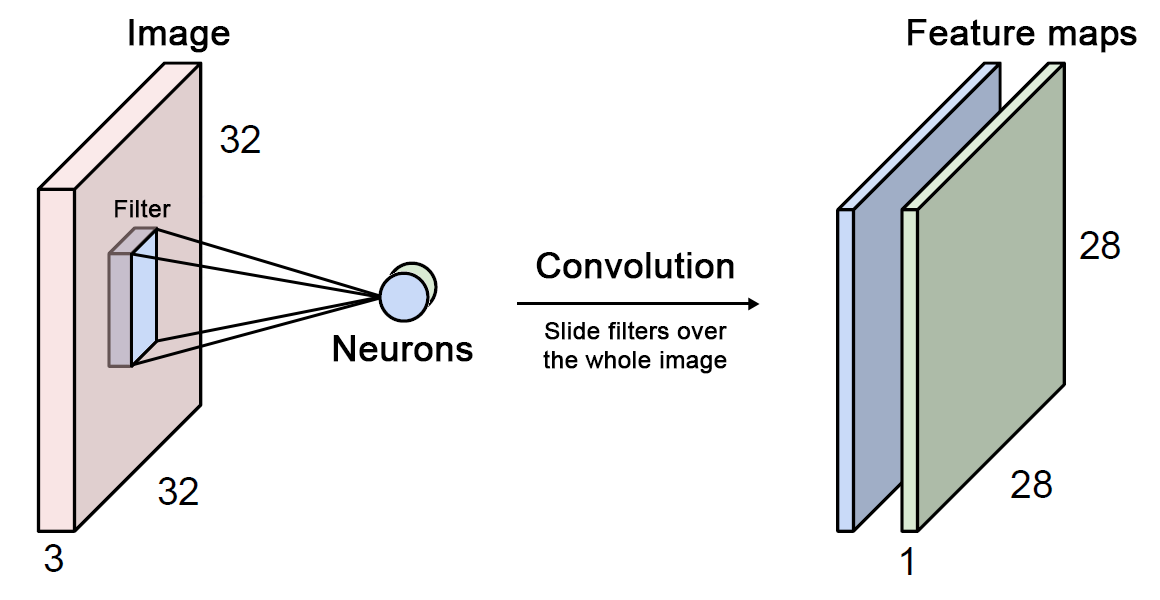
\includegraphics[width=\textwidth]{gfx/conv-layer-2}
  \end{center}
  \caption{}
  \label{fig:sec:concepts:conv-net}
\end{figure}


\todo[inline]{TODO}
Summarizing, CNNs are mainly composed by \todo{?}N types of layers: Convolutional layers, pooling layers, ReLU layers, fully connected layers.
Convolutional layers perform feature detection.
Pooling layers reduce the dimensionality of feature maps.
ReLU layers \todo{?}?.
Fully connected layers perform classification.

\subsection{Layers}
\label{sub:concepts:convolutional-neural-networks:layers}

\makeatletter
\renewcommand\paragraph{\@startsection{paragraph}{4}{\z@}%
  {-3.25ex \@plus -1ex \@minus -0.2ex}%
  {0.01pt}%
  {\raggedsection\normalfont\sectfont\nobreak\size@paragraph}%
}
\makeatother


For easier reference in Chapter \ref{sec:system}, here's a list of useful concepts in CNNs:

\begin{description}


  \item[Kernel]
  A kernel, also called filter or mask, is an image transformation matrix, usually small. The matrix gets applied convolutionally

  \item[Receptive field]
  The size of the filter.

  \item[Convolutional filter]
  Also called perceptive field
  TODO
  \todo[inline]{}
\end{description}

In image processing it can be understood as a sliding window of ${N}\times{N}$ pixels, the filter, that gets applied to every single pixel of the original image and produces a new image (often called feature map) that captures either edges, straight lines, etc.
For the convolution to capture features of a pixel the filter has to take into account neighboring pixels.




% ------------------------------------------------------------------------------

\section{Non-linear transformations}
\label{sec:Non-linear transformations}

They are filters (a.k.a. kernel or feature map), often represented by $\phi$, implemented as functions whose output is not linear to its input often used for feature extraction on images (edges, connectivity, etc.). Perceptron neurons use these as activation function because the dimensionality of the input can be reduced so that it becomes binary classifiable.

\begin{description}
  \item[tanh]
  \item[ReLU]
\end{description}
